\section{Auswertung des \qlearning Agenten}
In den folgenden Abschnitten werden die Ergebnisse der Q-Learning Agenten vorgestellt und ausgewertet. Zunächst wird die Konvergenz während dem Training und die Spielstärke betrachtet. Anschließend wird vorgestellt, welche Auswirkung die Nutzung von Afterstates hat. Abschließend erfolgt eine Detailbetrachtung für ausgewählte Zustände.

\subsection{Konvergenz der Rate optimaler Aktionen}
\begin{figure}
\centering
\begin{subfigure}[b]{0.75\textwidth}
    \centering
   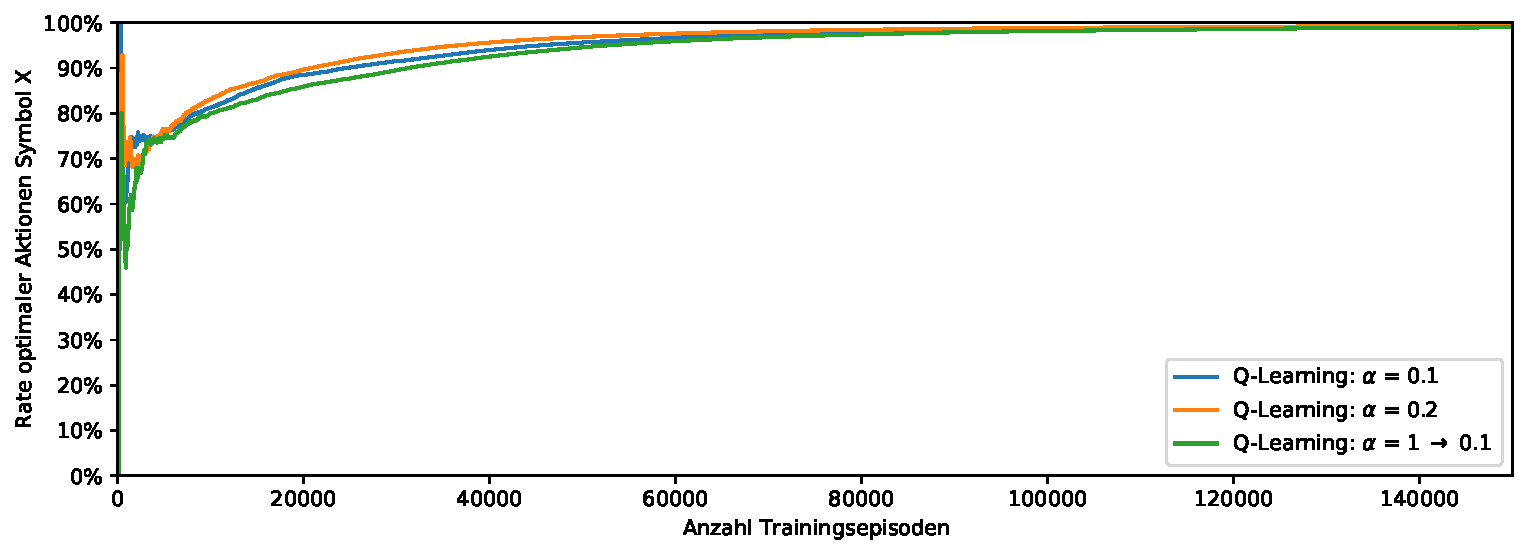
\includegraphics[width=1\linewidth]{convergence/convergence_compare_alpha_QLearning_X.pdf}
   \caption{Symbol X}
   \label{fig:convergence_compare_alpha_QLearning_X} 
\end{subfigure}

\begin{subfigure}[b]{0.75\textwidth}
    \centering
   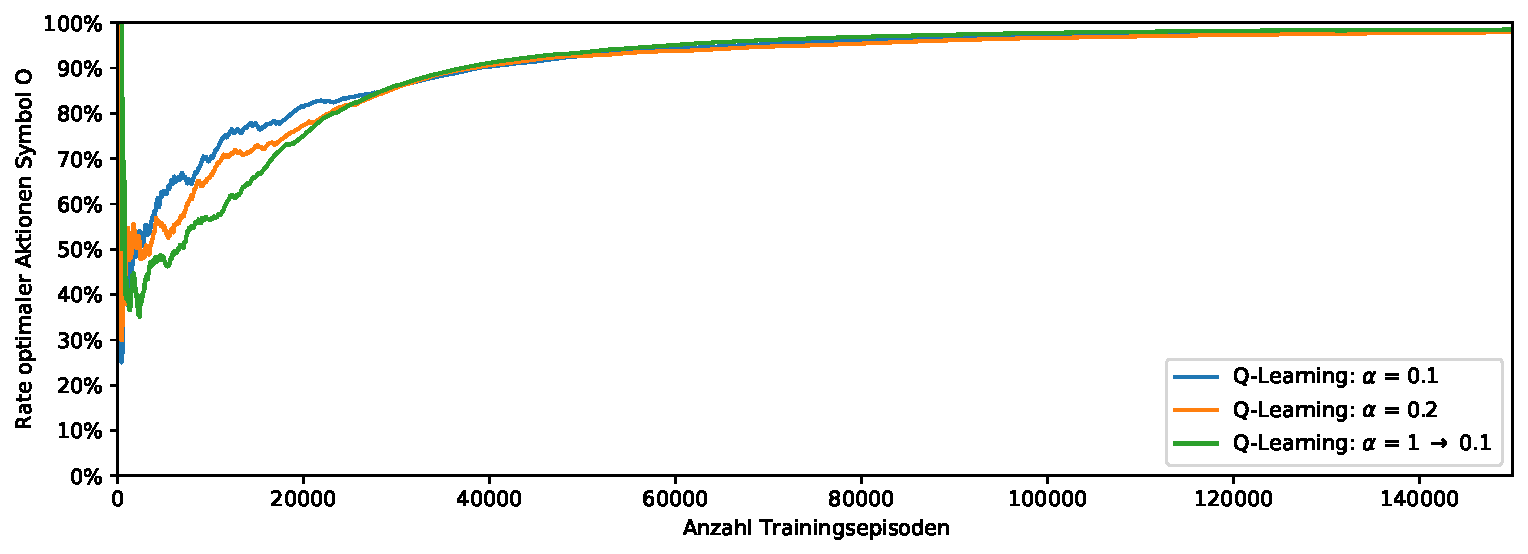
\includegraphics[width=1\linewidth]{convergence/convergence_compare_alpha_QLearning_O.pdf}
   \caption{Symbol O}
   \label{fig:convergence_compare_alpha_QLearning_O}
\end{subfigure}

\caption[Rate optimaler Aktionen Q-Learning unterschiedliche Lernraten, klassisches \splay]{Rate optimaler Aktionen von Q-Learning für verschiedene Lernraten $\alpha$, klassisches \splay (a) Symbol X (b) Symbol O}
\label{fig:convergence_compare_alpha_QLearning}
\end{figure}


\cref{fig:convergence_compare_alpha_QLearning} zeigt den Verlauf der Rate optimaler Aktionen der \qlearning Agenten mit den drei verschiedenen Lernraten $\alpha$ währen des Trainings mit klassischem \splay. 
Die drei Graphen für Symbol X unterscheiden sich stärker innerhalb der ersten 5.000 Episoden. 
Ab ungefähr 70.000 Episoden ist die Rate stabil, wobei $\alpha = 0,2$ am schnellsten konvergiert, dicht gefolgt von $\alpha=0,1$. 
Im Gegensatz dazu unterscheiden sich die Graphen für Symbol O deutlich stärker und verlaufen erst ab ungefähr 30.000 Episoden gleich. 
Zudem beginnt die Rate für Symbol O etwas über 0,4 und ist somit niedriger als die Rate von X.
Dies kann erklärt werden durch die unterschiedliche Wahrscheinlichkeit zufällig eine optimale Aktion zu wählen, wie \cref{sec:vergleichswerte} beschrieben. 
Ab ungefähr 100.000 Episoden stabilisiert sich die Rate für das Symbol O auf einem niedrigeren Wert als X. 
Somit konvergiert Symbol O langsamer als Symbol X, wobei Symbol O für $\alpha = 0,1$  am schnellsten konvergiert. 
Da die Agenten durch \splay trainiert werden und somit beide Symbole spielen, muss die Konvergenzrate auch für beide Symbole gemeinsam betrachtet werden. 
Daher konvergiert \qlearning bei klassischem \splay für $\alpha=0,1$ am schnellsten. 

Der Vergleich der Rate optimaler Aktionen von \qlearning für alternierendes \splay ist im \cref{chap:app_qlearning}. 
Für beide Symbole konvergiert alternierendes \splay langsamer als das klassische \splay und stabilisiert sich auf einer geringeren Rate.

\subsection{Spielstärke}

\cref{tab:playingAbility_ql_normal} und \cref{tab:playingAbility_ql_alternate} zeigen die durchschnittliche Spielstärke der trainierten Agenten für klassisches und alternierendes \splay. 
Alle Agenten, die mit klassischem \splay trainiert wurden, erreichen eine bessere durchschnittliche Spielstärke als Minimax. 
Im Gegensatz dazu ist die durchschnittliche Spielstärke aller Agenten, die mit alternierendem \splay trainiert wurden schlechter als die des Minimax und deutlich schlechter im Vergleich zum klassischen \splay.

Der \qlearning Agent, der die Lernrate $\alpha=0,1$ nutzt und mit klassischem \splay trainiert wurde, konvergierte am schnellsten und erreicht mit durchschnittlich 8.002,72 die höchste Spielstärke.
\cref{tab:resultmatrix_ql_normal_alpha01} enthält die Spielergebnisse der Evaluationsspiele dieses Agenten. 
Der Agent spielt perfekt gegen Minimax sowohl als Symbol X als auch Symbol O. 
Gegen Random verliert der Agent keine Spiele und erreicht eine Gewinnrate als Symbol X von 99\% und Symbol O von 91\%. 
Die Gewinnrate ist somit besser als die von Minimax, die 97\% bzw. 78\% beträgt. 
Somit konnte \qlearning durch \splay lernen, \ac{TTT} gegen Gegner unterschiedlicher Spielstärke erfolgreich zu spielen. 
Die Spielergebnismatrizen des \qlearning Agenten für die anderen Hyperparameter und Arten von\splay sind im \cref{chap:app_qlearning} angegeben.

\begin{table}
\centering
\caption[Spielstärke Q-Learning unterschiedliche Lernraten, klassisches \splay]{Spielstärke von Q-Learning mit unterschiedlichen Lernraten, klassisches \splay}
\label{tab:playingAbility_ql_normal}

% change color with \textcolor{red}{text}
\begin{tabular}{lrrr}
\toprule
Lernrate $\alpha$ &  Spielst"arke Q-Learning & Spielst"arke Minimax & Differenz zu Minimax \\ \midrule
Konstant 0,1                    & 8.002,72 $\pm$ \phantom{0}30,03   & 6.917,86  & 1.084,86 $\pm$ \phantom{0}30,03 \\
Konstant 0,2                    & 7.801,36 $\pm$ 131,22             & 6.917,86  & 883,5 $\pm$ 131,22 \\
Abnehmend 1 $\rightarrow$ 0,1   & 7.894,92 $\pm$ 132,52             & 6.917,86  & 977,06 $\pm$ 132,52 \\ \bottomrule

\end{tabular}

\end{table}
\begin{table}
\centering
\caption[Spielstärke Q-Learning unterschiedliche Lernraten, alternierendes \splay]{Spielstärke von Q-Learning mit unterschiedlichen Lernraten, alternierendes \splay}
\label{tab:playingAbility_ql_alternate}

\begin{tabular}{lrrr}
\toprule
Lernrate $\alpha$ &  Spielst"arke Q-Learning & Spielst"arke Minimax & Differenz zu Minimax \\ \midrule
Konstant 0,1                    & 6.465,66 $\pm$ 481,99             & 6.917,86  & \textcolor{red}{-452,2 $\pm$ 481,99} \\
Konstant 0,2                    & 6.904,92 $\pm$ 399,15             & 6.917,86  & \textcolor{red}{-12,94 $\pm$ 399,15} \\
Abnehmend 1 $\rightarrow$ 0,1   & 6.110,56 $\pm$ 224,66             & 6.917,86  & \textcolor{red}{-807,3 $\pm$ 224,66} \\ \bottomrule

\end{tabular}
\end{table}
\begin{table}
\centering
\caption[Spielergebnismatrix \qlearning: $\alpha=0,1$, klassisches \splay]{Spielergebnismatrix für \qlearning mit Lernrate $\alpha=0,1$, klassisches \splay}
\label{tab:resultmatrix_ql_normal_alpha01}

\begin{tabular}{llrlr}
\toprule
 & \multicolumn{2}{l}{\textbf{Minimax}} & \multicolumn{2}{l}{\textbf{Random}} \\ \midrule
\textbf{X Q-Learning}   & X Q-Learning:     & 0,00\% $\pm$    0,00\%            & X Q-Learning:         & 99,22\% $\pm$ 0,37\%  \\
                        & O Minimax:        & 0,00\% $\pm$    0,00\%            & O Random:            & 0,00\% $\pm$ 0,00\%  \\
                        & Unentschieden:    & 100,00\% $\pm$  0,00\%            & Unentschieden:        & 0,78\% $\pm$ 0,37\%  \\ \cmidrule{2-5}
\textbf{O Q-Learning}   & X Minimax:        & 0,00\% $\pm$    0,00\%            & X Random:             & 0,00\% $\pm$ 0,00\%  \\
                        & O Q-Learning:     & 0,00\% $\pm$    0,00\%            & O Q-Learning:         & 91,45\% $\pm$ 0,21\%  \\
                        & Unentschieden:    & 100,00\% $\pm$  0,00\%            & Unentschieden:        & 8,55\% $\pm$ 0,21\%  \\ \bottomrule
\end{tabular}
\end{table}

\subsection{\wtable}
Zur Evaluation der Auswirkung von Afterstates auf die Konvergenz und Spielstärke wird der stärkste ermittelte \qlearning Agent mit einem Agenten verglichen, der eine \wtable und die gleichen Hyperparameter nutzt. 
Wie im vorigen Abschnitt beschrieben, ist dies ein \qlearning Agent mit Lernrate $\alpha=0,1$, der mit klassischen \splay trainiert wird.

\cref{fig:convergence_compare_experience_QLearning} vergleicht die Rate optimaler Aktionen von Agenten mit \qtable und mit \wtable. 
Sowohl für Symbol X als auch Symbol O konvergiert der Agent mit \wtable deutlich schneller und stabilisiert sich auf einer höheren Rate optimaler Aktionen. 
Dies äußert sich in der Spielstärke des Agenten, wie \cref{tab:resultmatrix_ql_normal_alpha01_afterstate} zeigt.

Durch die Nutzung des \wtable im Vergleich zur \qtable steigert sich die durchschnittliche Gewinnrate gegen Random als Symbol X von 99,22\% auf 99,46\% und als Symbol O von 91,45\% auf 91,51\%.
Die absolute Spielstärke steigt von 8.002,72 auf 8.036,68. 
Dies könnte wie in \cref{sec:afterstates} und \cite[S. 136f.]{suttonReinforcementLearningIntroduction2018} beschrieben, auf die effektivere Nutzung der gesammelten Erfahrung zurückgeführt werden.
Da die Spielstärke der Spielstärke für den \qtable jedoch $\pm 75,69$ beträgt und die Stichprobenanzahl mit $N=5$ klein ist, kann dies nicht sicher gesagt werden.
Es ist daher auch möglich, dass die Verbesserung durch Zufall entstanden somit statistisch nicht signifikant ist.

Die ermittelten Spielergebnisse des \qlearning Agenten sind konsistent mit anderen Experimenten in \cite{mirnovi.QLearningTicTacToe2020}. 
In diesen wurde jedoch ein Double \qlearning Agent mit \qtable und abnehmenden Hyperparametern durch klassisches Self-play für 3.000.000 Episoden trainiert.

\begin{figure}
\centering
\begin{subfigure}[b]{0.75\textwidth}
    \centering
   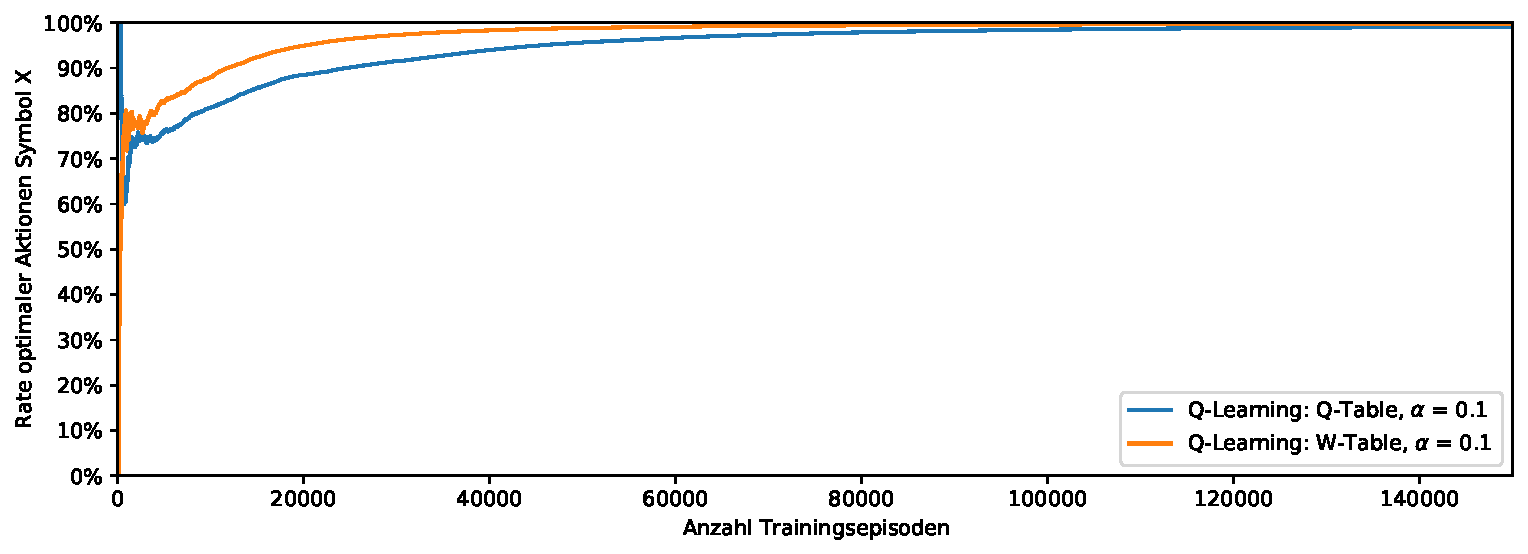
\includegraphics[width=1\linewidth]{convergence/convergence_compare_experience_QLearning_X.pdf}
   \caption{Symbol X}
   \label{fig:convergence_compare_experience_QLearning_X} 
\end{subfigure}

\begin{subfigure}[b]{0.75\textwidth}
    \centering
   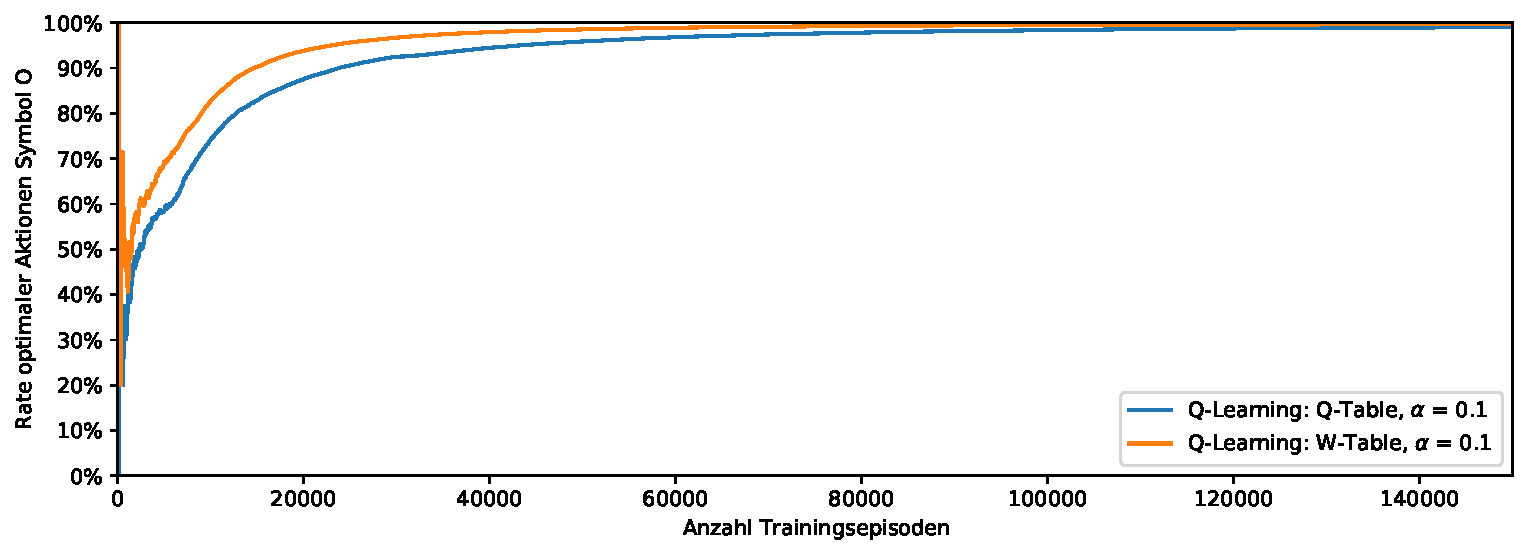
\includegraphics[width=1\linewidth]{convergence/convergence_compare_experience_QLearning_O.pdf}
   \caption{Symbol O}
   \label{fig:convergence_compare_experience_QLearning_O}
\end{subfigure}

\caption[Rate optimaler Aktionen bester Q-Learning Agent, \wtable, klassisches \splay]{Rate optimaler Aktionen von Q-Learning Lernrate $\alpha=0,1$, \wtable, klassisches \splay (a) Symbol X (b) Symbol O}
\label{fig:convergence_compare_experience_QLearning}
\end{figure}

\begin{table}
\centering
\caption[Spielergebnismatrix Q-Learning: $\alpha=0,1$, \wtable, klassisches \splay]{Spielergebnismatrix für \qlearning mit Lernrate $\alpha=0,1$ und \wtable, klassisches \splay}
\label{tab:resultmatrix_ql_normal_alpha01_afterstate}

\begin{tabular}{llrlr}
\toprule
 & \multicolumn{2}{l}{\textbf{Minimax}} & \multicolumn{2}{l}{\textbf{Random}} \\ \midrule
\textbf{X Q-Learning}   & X Q-Learning:     & 0,00\% $\pm$    0,00\%            & X Q-Learning:         & 99,46\% $\pm$ 0,05\%  \\
                        & O Minimax:        & 0,00\% $\pm$    0,00\%            & O Random:            & 0,00\% $\pm$ 0,00\%  \\
                        & Unentschieden:    & 100,00\% $\pm$  0,00\%            & Unentschieden:        & 0,54\% $\pm$ 0,05\%  \\ \cmidrule{2-5}
\textbf{O Q-Learning}   & X Minimax:        & 0,00\% $\pm$    0,00\%            & X Random:             & 0,00\% $\pm$ 0,00\%  \\
                        & O Q-Learning:     & 0,00\% $\pm$    0,00\%            & O Q-Learning:         & 91,51\% $\pm$ 0,20\%  \\
                        & Unentschieden:    & 100,00\% $\pm$  0,00\%            & Unentschieden:        & 8,49\% $\pm$ 0,20\%  \\ \bottomrule
\end{tabular}
\end{table}

\subsection{Detailbetrachtung}
Die Spielstärke des \qlearning Agenten wirft die Frage auf, wie der Agent besser als ein Minimax-Algorithmus spielen kann. 
Wie in \cref{sec:minimax} erwähnt, erwartet der  Minimax-Algorithmus einen optimalen Gegner und spielt nur gegen diesen optimal. 
Hingegen hat \qlearning auch gelernt gegen nicht optimale Gegner optimal zu spielen.
Dies wird deutlich, wenn die Einträge der \qtable \bzw \wtable für einen Zustand betrachtet werden. 
\cref{ttt_boards/ttt_6754} zeigt das Spielfeld des Zustands $6754$ und \cref{tab:state6754} die Bewertung der legalen Aktionen durch den Minimax und \qlearning Agent mit \wtable. 
In diesem Zustand ist Symbol X am Zug und die laut Expert Play optimalen Aktionen sind 4 und 8, um den Gegner zum Blocken zu zwingen. 
Wählt Symbol O im nächsten Zug die nicht optimale Aktion 7, gewinnt X. 
Die Aktion 7 garantiert hingegen, dass das Spiel unentschieden endet. 
Minimax weist allen Aktionen den Wert 0 zu, da dieser von einem optimalen Gegner und somit einem Unentschieden ausgeht. 
Der \qlearning Agent weist den Aktionen 4 und 8 einen positiven Wert zu, da im Rahmen des Trainings auch gegen nicht optimale Gegner gespielt wurde und so Erfahrungen vorliegen, in denen der Agent das Spiel aus diesem Zustand gewonnen hat. 

\begin{minipage}{\textwidth}
  \begin{minipage}[b]{0.49\textwidth}
    \centering
    \captionsetup{type=figure}
    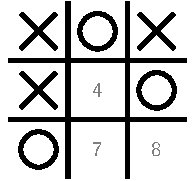
\includegraphics[]{ttt_boards/ttt_6754.pdf}
    \captionof{figure}{Spielfeldkonstellation Zustand 6754}
    \label{ttt_boards/ttt_6754}
  \end{minipage}
  \hfill
  \begin{minipage}[b]{0.49\textwidth}
    \centering
        \captionsetup{type=table}
    %\begin{table}
%\centering
%\caption{Bewertung Aktionen in State $6754_{10}$ bester Q-Learning Agent mit Lernrate $\alpha$ =0,1 und W-Table}
\begin{tabular}{lll}
\toprule
Aktion  & Minimax & Q-Learning \\ \midrule
4	    & 0	                & 0,0015 \\
7   	& 0	                & 0,0000 \\
8	    & 0	                & 0,0006 \\ \bottomrule
\end{tabular}
%\end{table}
    \captionof{table}{Bewertung Aktionen in Zustand 6754}
    \label{tab:state6754}
    \end{minipage}
\end{minipage}

Eine Forschungsfrage ist die Ermittlung der besten ersten Aktion für das Symbol X. 
Zur Beantwortung soll die Bewertung des besten \qlearning Agenten für alle legalen Aktionen im Zustand $0$ betrachtet werden. 
\cref{tab:state0_eval_ql} listet die durchschnittliche Bewertung der Aktionen von fünf \qlearning Agenten mit \wtable. 
Die Aktion 4 (Mitte) hat mit 0,0053 den höchsten \qValue. 
Jedoch zeigt die Auflistung der \qValues ein weiteres Problem.  
Die Tabelle enthält jeweils vier Bewertungen für Ecken und Kanten, die alle den gleichen Wert haben sollten. 
Die Aktionen sollten den gleichen Wert haben, da sie in Zuständen resultieren, die nach Rotation oder Spiegelung äquivalent sind. 
Durch Berechnung der durchschnittlichen Bewertung je äquivalenter Aktion, wie in \cref{tab:state0_eval_ql_aggregated}, kann die durchschnittliche Rangfolge der Aktionen angegeben werden. 
Demnach ist die Aktion Mitte weiterhin die beste Aktion, gefolgt von der Aktion Ecke. 
Für eine abschließende Beantwortung der Frage wäre eine Enkodierung der Zustände notwendig, die äquivalenten Zuständen einen gemeinsamen Bezeichner und \qValue zuweist. 
Das Ergebnis, dass die beste erste Aktion die Mitte ist, ist jedoch konsistent zu vorher durchgeführten Experimenten von \cite{kutscheraa.BestOpeningMove2018}.

\begin{table}[!htb]
    \begin{minipage}[t]{.5\textwidth}
        \centering
        \caption{Bewertung Zustand 0 \\ bester Q-Learning Agent}
        \label{tab:state0_eval_ql}
        \begin{tabular}{lr}
        \toprule
        Aktion  & Bewertung \\ \midrule
        0       & 0,0041 \\
        1       & 0,0041 \\
        2		& 0,0045 \\
        3		& 0,0033 \\
        4		& 0,0053 \\
        5		& 0,0030 \\
        6		& 0,0035 \\
        7		& 0,0033 \\
        8		& 0,0044 \\ \bottomrule
    \end{tabular}
    \end{minipage}%
    \begin{minipage}[t]{.5\textwidth}
        \centering
        \caption{Bewertung Aktionsklassen Zustand 0 bester Q-Learning Agent}
        \label{tab:state0_eval_ql_aggregated}
        \begin{tabular}{lr}
        \toprule
        Aktion  & Bewertung \\ \midrule
        Ecke	& 0,0041 \\
        Kante	& 0,0034 \\
        Mitte	& 0,0053 \\ \bottomrule
        \end{tabular}
    \end{minipage}
\end{table}